\subsection{1. Thiết kế hệ thống}
\indent\indent Quy trình tổng quát của hệ thống được minh họa tại \textbf{Hình \ref{fig:LXLTongQuat}}, bao gồm 4 giai đoạn xử lý tuần tự: (1) Phân tách video, (2) Tiền xử lý và trích xuất đặc trưng, (3) Xây dựng MG, và (4) Suy luận phân tầng.

\begin{figure}[H]
    \centering
    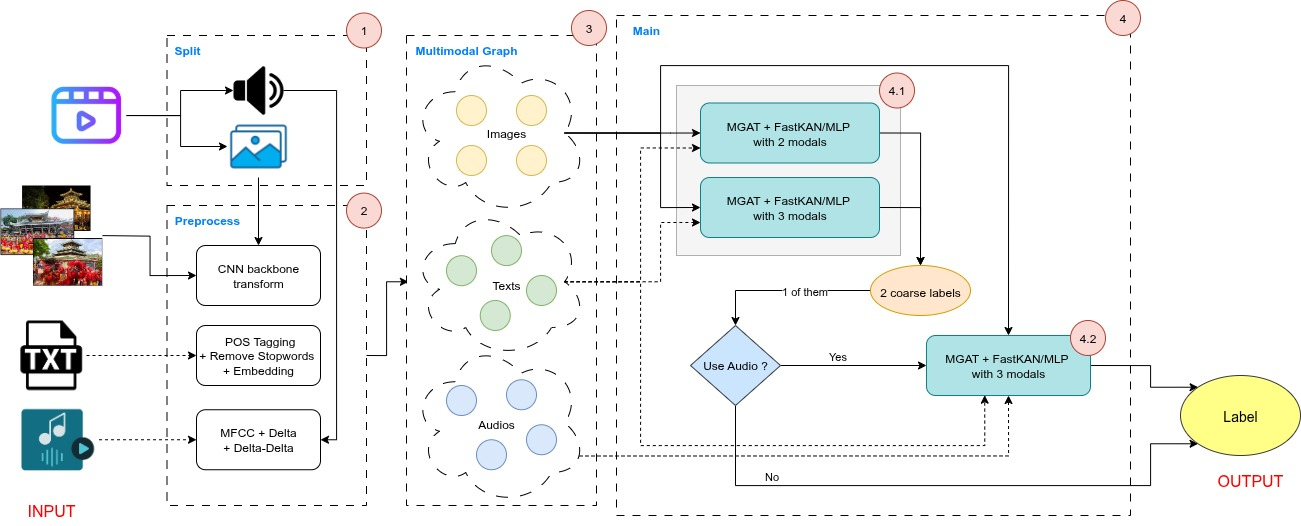
\includegraphics[width=\linewidth]{images/part-02/chap-02/sec-01/TongQuat.jpg}
    \vspace{0.3cm}
    \caption{Luồng xử lý tổng quát của hệ thống khi triển khai thành ứng dụng}
    \label{fig:LXLTongQuat}
\end{figure}

\indent\textbf{Đặc tả Dữ liệu đầu vào (INPUT):} Hệ thống được thiết kế với cơ chế chấp nhận thiếu hụt, cho phép hoạt động ngay cả khi người dùng không cung cấp đầy đủ văn bản hoặc âm thanh. Tuy nhiên, dữ liệu hình ảnh là thành phần bắt buộc. Các ràng buộc cụ thể bao gồm:\vspace{-0.1cm}
\begin{itemize}[label={--}, itemsep=1pt]
    \item \textbf{Video:} Yêu cầu thời lượng tối thiểu 30 giây và tối đa 2 phút. Trong trường hợp người dùng đã cung cấp đủ tối thiểu 3 hình ảnh hợp lệ, việc tải lên video trở thành tùy chọn.
    \item \textbf{Hình ảnh:} Số lượng tối thiểu là 3 và tối đa 20 ảnh. Nếu video hợp lệ đã được tải lên, hệ thống sẽ tự động trích xuất khung hình và người dùng không cần thao tác thêm.
    \item \textbf{Văn bản:} Đây là thành phần tùy chọn. Nếu cung cấp, hệ thống chấp nhận duy nhất 01 tệp tin định dạng \texttt{.txt} chứa nội dung mô tả.
    \item \textbf{Âm thanh:} Đây cũng là thành phần tùy chọn. Hệ thống chấp nhận 01 tệp tin định dạng \texttt{.mp3} hoặc \texttt{.wav} với thời lượng từ 30 giây đến 2 phút. Trường hợp người dùng tải lên video, phần âm thanh sẽ được tự động tách xuất từ video đó.
\end{itemize}

\textbf{Dữ liệu đầu ra (OUTPUT):} Nhãn chủ đề ICH được dự đoán bởi mô hình, kèm theo độ tin cậy.\vspace{0.3cm}

\newpage
\indent\textbf{Chi tiết các giai đoạn xử lý:}
\begin{itemize}[label={--}, itemsep=3pt]
    \item \textbf{Giai đoạn 1 -- Phân tách video:} Nếu người dùng có tải lên video đầu vào, hệ thống sẽ tiến hành phân tách, quá trình này thực hiện trích xuất chuỗi hình ảnh (tần suất 4 giây/khung hình) và các đoạn âm thanh (5 giây/đoạn) để chuẩn bị cho bước tiếp theo.

    \item \textbf{Giai đoạn 2 -- Tiền xử lý và trích xuất đặc trưng:} Các dữ liệu thô ứng với mỗi phương thức sẽ có cách xử lý riêng biệt khác nhau, bao gồm:
    \begin{itemize}[label={+}, itemsep=1pt]
        \item \textbf{Đặc trưng hình ảnh:} Hệ thống tích hợp 6 kiến trúc CNN tiên tiến đã được huấn luyện trước trên tập dữ liệu ImageNet làm bộ trích xuất đặc trưng nền tảng (backbone). Người dùng có quyền lựa chọn một trong các mô hình: \textbf{ResNet18}, \textbf{RegNetX400MF}, \textbf{MobileNetV3 Large}, \textbf{MobileNetV3 Small}, \textbf{DenseNet121} hoặc \textbf{ShuffleNetV2 1.0x}. Hình ảnh đầu vào được tự động thay đổi kích thước (resize) và chuẩn hóa (normalize) tuân theo chuẩn của backbone được chọn.
        
        \item \textbf{Đặc trưng văn bản:} Dữ liệu văn bản trải qua quy trình gán nhãn từ loại (POS Tagging) sử dụng thư viện \textit{underthesea} chuyên dụng cho tiếng Việt. Sau đó, hệ thống tiến hành loại bỏ stopwords và chỉ giữ lại các từ mang nội dung chính thuộc các nhóm: danh từ ($N$), danh từ riêng ($Np$) động từ ($V$) và tính từ ($A$). Để biểu diễn ngữ nghĩa, hệ thống sử dụng mô hình \textbf{all-MiniLM-L6-v2} nhằm chuyển đổi cặp {từ khóa, câu chứa từ khóa} thành vector embedding ngữ nghĩa.
        
        \item \textbf{Đặc trưng âm thanh:} Hệ thống áp dụng kỹ thuật trích xuất MFCC để nắm bắt đặc trưng phổ âm. Để mô tả sự biến thiên của tín hiệu âm thanh theo thời gian (yếu tố quan trọng trong các lễ hội âm nhạc), hệ thống kết hợp thêm các đặc trưng động là Delta (đạo hàm bậc 1) và Delta-Delta (đạo hàm bậc 2).
    \end{itemize}

    \item \textbf{Giai đoạn 3 -- Xây dựng MG:}  Các vector đặc trưng từ ba nguồn dữ liệu được chuyển đổi thành các đỉnh trong một đồ thị thống nhất. Về mặt cấu trúc, đây là đồ thị đa phương thức cấp đỉnh (Node-Level MG). Trong đó, các kết nối được thiết lập giữa tất cả các đỉnh, bao gồm các đỉnh cùng phương thức và các đỉnh khác phương thức (ví dụ: kết nối giữa 1 đỉnh hình ảnh và 1 đỉnh văn bản). Trọng số của các kết nối này là tham số học được (learnable parameters), bằng việc huấn luyện các mô hình \textbf{Giai đoạn 4}, nhằm tìm ra cấu trúc tương quan tốt nhất.

    \item \textbf{Giai đoạn 4 -- Suy luận phân tầng:} Đây là cơ chế ra quyết định được thiết kế nhằm tối ưu hóa việc sử dụng dữ liệu âm thanh. Hệ thống sử dụng song song hai mô hình MGAT + FastKAN/MLP gồm: mô hình được huấn luyện chỉ trên 2 phương thức (hình ảnh và văn bản) và mô hình được huấn luyện trên cả 3 phương thức (hình ảnh, văn bản và âm thanh).
    \begin{itemize}[label={+}, itemsep=1pt]
        \item \textbf{Bước 4.1 -- Dự đoán nhãn thô:} Hệ thống tiến hành dùng 2 mô hình MGAT + FastKAN/MLP đã đề cập ở bên trên để dự đoán và cho ra 2 nhãn thô.
        
        \item \textbf{Bước 4.2 -- Ra quyết định:} Dựa trên nhãn thô, hệ thống tiến hành xét rằng liệu 1 trong số các nhãn dự đoán được có dùng âm thanh hay không, cụ thể như sau: 
        \begin{itemize}[label={\textbullet}, itemsep=1pt]
            \item \textbf{Trường hợp Có (Yes):} Hệ thống sử dụng dữ liệu hình ảnh, văn bản cùng với âm thanh để đưa vào mô hình MGAT + FastKAN/MLP (3 phương thức) một lần nữa, nhằm dự đoán ra kết quả cuối cùng.
            \item \textbf{Trường hợp Không (No):} Hệ thống sẽ ưu tiên nhãn thô có độ tin cậy cao hơn giữa 2 nhãn để cho ra kết quả cuối cùng.
        \end{itemize}
    \end{itemize}
\end{itemize}

\subsubsection{1.1. Mô hình CNN baseline:}
\indent\indent Trước khi đi vào xây dựng mô hình MGAT + FastKAN/MLP, tôi tiến hành xây dựng và huấn luyện một kiến trúc CNN cơ sở (baseline) chỉ sử dụng dữ liệu hình ảnh. Mục tiêu của bước này là tạo ra một mốc hiệu năng tham chiếu (benchmark) để đánh giá sự cải thiện của các phương pháp đa phương thức sau này.\vspace{0.3cm}

\indent Kiến trúc của mô hình CNN baseline được minh họa tại \textbf{Hình \ref{fig:KTCNNBaseline}}, bao gồm các thành phần và cơ chế hoạt động như sau:
\begin{figure}[H]
    \centering
    \scalebox{0.6}{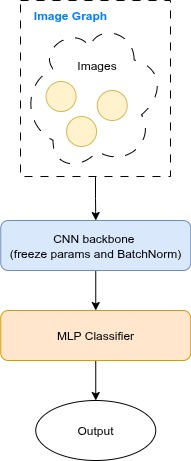
\includegraphics{images/part-02/chap-02/sec-01/CNNBaseline.jpg}}
    \vspace{0.3cm}
    \caption{Kiến trúc của mô hình CNN baseline}
    \label{fig:KTCNNBaseline}
\end{figure}

\textbf{Đầu vào (Image Graph):} Đây là dữ liệu ảnh đã được tiền xử lý bằng cách dùng các transforms từ các CNN backbone tương ứng.\vspace{0.3cm}

\textbf{Đầu ra (Output):} Kết quả dự đoán xác suất cho từng hình ảnh, sau đó tiền hành lấy trung bình cộng xác suất lại và cho ra kết quả phân lớp cuối cùng trên một mẫu đồ thị.\vspace{0.3cm}

\newpage
\textbf{Quy trình xử lý:}\vspace{-0.1cm}
\begin{itemize}[label={--}, itemsep=3pt]    
    \item \textbf{Trích xuất đặc trưng:} Tôi sử dụng 6 kiến trúc CNN bao gồm \textbf{ResNet18}, \textbf{RegNetX400MF}, \textbf{MobileNetV3 Large}, \textbf{MobileNetV3 Small}, \textbf{DenseNet121} và \textbf{ShuffleNetV2 1.0x} đã được huấn luyện trước trên tập dữ liệu khổng lồ ImageNet. Điểm quan trọng trong thiết kế này là cơ chế "đóng băng" (freezing):
    \begin{itemize}[label={+}]
        \item \textbf{Freeze Parameters:} Toàn bộ trọng số và bias của các lớp tích chập được giữ nguyên, không cập nhật trong quá trình lan truyền ngược. Điều này giúp bảo toàn khả năng nhận diện các đặc trưng cơ bản (cạnh, góc, textur) mà mạng đã học được từ ImageNet.
        \item \textbf{Freeze BatchNorm:} Các lớp Batch Normalization cũng được chuyển sang chế độ đánh giá (\textit{eval mode}), nghĩa là chúng sử dụng các giá trị trung bình (mean) và phương sai (variance) toàn cục đã học trước đó thay vì tính toán lại trên từng batch dữ liệu huấn luyện mới. Điều này đảm bảo tính ổn định của đặc trưng đầu ra.
    \end{itemize}
    
    \item \textbf{Bộ phân lớp (MLP Classifier):}  Các đặc trưng sau khi đi qua Backbone sẽ được đưa vào một mạng MLP. Đây là thành phần duy nhất có thể học được. Nhiệm vụ của MLP là học cách ánh xạ từ không gian đặc trưng của ImageNet sang không gian nhãn của ICH.
\end{itemize}
\subsubsection{1.2. Mô hình MGAT + FastKAN/MLP}
%===================================================================
\paragraph{1.2.1. Tầng trích xuất đặc trưng}
\indent\indent Đây là tầng đầu tiên tiếp nhận dữ liệu từ ba phương thức khác nhau. Kiến trúc của tầng này được minh họa tại \textbf{Hình \ref{fig:KTExtractFeaturesLayers}}, bao gồm ba nhánh xử lý độc lập:\vspace{-0.1cm}
\begin{itemize}[label={--}, itemsep=1pt]
    \item \textbf{Image Extractor:} Sử dụng backbone CNN đã được đóng băng tham số và BatchNorm để trích xuất đặc trưng hình ảnh. Đầu ra từ backbone được đưa qua một tầng Linear để chiếu về chiều không gian vector mong muốn (448 chiều).
    \item \textbf{Text Extractor:} Kết hợp vector embedding của từ (Word) và câu (Sentence).
    \item \textbf{Audio Extractor:} Xử lý đặc trưng MFCC kết hợp với các giá trị Delta và Delta-Delta.
\end{itemize}

\begin{figure}[H]
    \centering
    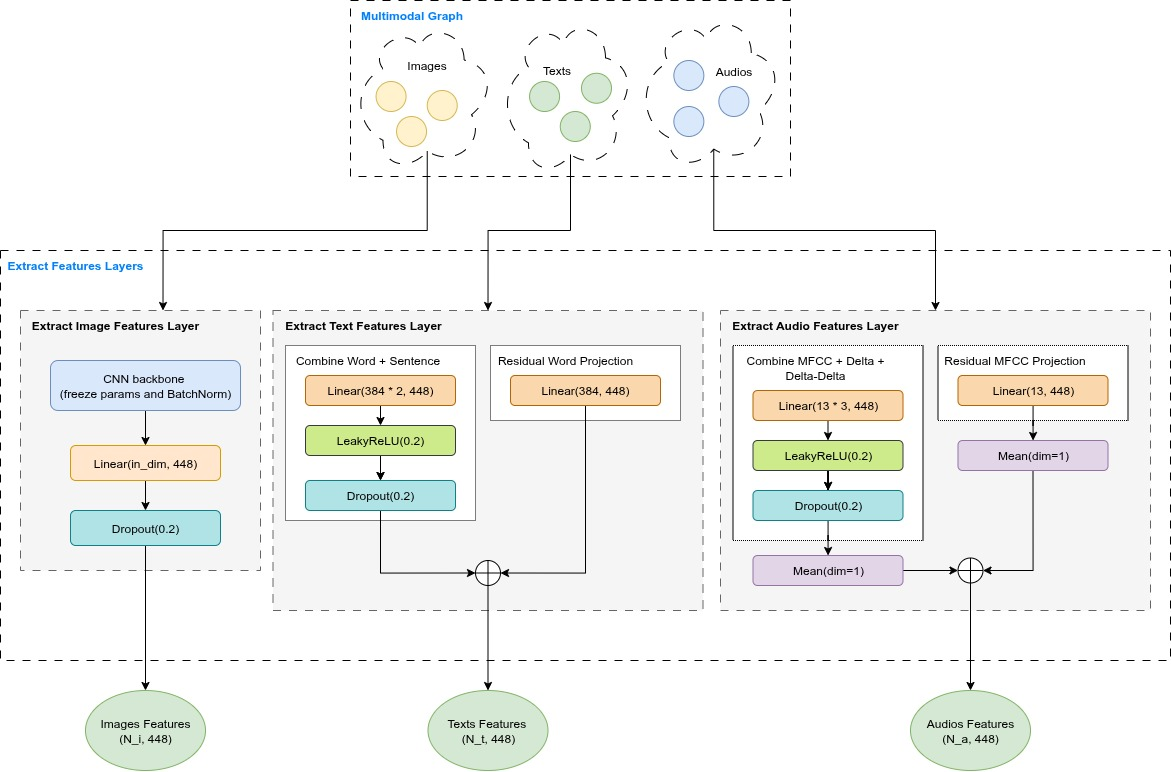
\includegraphics[width=\linewidth]{images/part-02/chap-02/sec-01/ExtractFeaturesLayers.jpg}
    \vspace{0.3cm}
    \caption{Kiến trúc chi tiết của Extract Features Layers}
    \label{fig:KTExtractFeaturesLayers}
\end{figure}

Đối với nhánh đặc trưng hình ảnh, do backbone đã cung cấp các vector đặc trưng giàu thông tin ngữ nghĩa, hệ thống chỉ áp dụng phép chiếu tuyến tính đơn giản. Ngược lại, đối với văn bản và âm thanh, hệ thống áp dụng cơ chế Residual Connection bằng cách cộng vector đặc trưng gốc (đã được chiếu về cùng chiều) vào đầu ra cuối cùng của nhánh. Kỹ thuật này giúp giải quyết vấn đề triệt tiêu đạo hàm khi huấn luyện mạng sâu, đồng thời bảo toàn thông tin gốc quan trọng trước các phép biến đổi phi tuyến có thể gây mất mát thông tin đặc trưng \cite{he2015deepresiduallearningimage}.
%===================================================================
\paragraph{1.2.2. Tầng chiếu không gian chung}
\indent\indent Mục tiêu của tầng này là đồng bộ hóa các vector đặc trưng từ ba phương thức khác nhau về cùng một không gian biểu diễn có số chiều cố định (512 chiều), với kiến trúc chi tiết tại \textbf{Hình \ref{fig:KTShareProjectionLayer}}.

\begin{figure}[H]
    \centering
    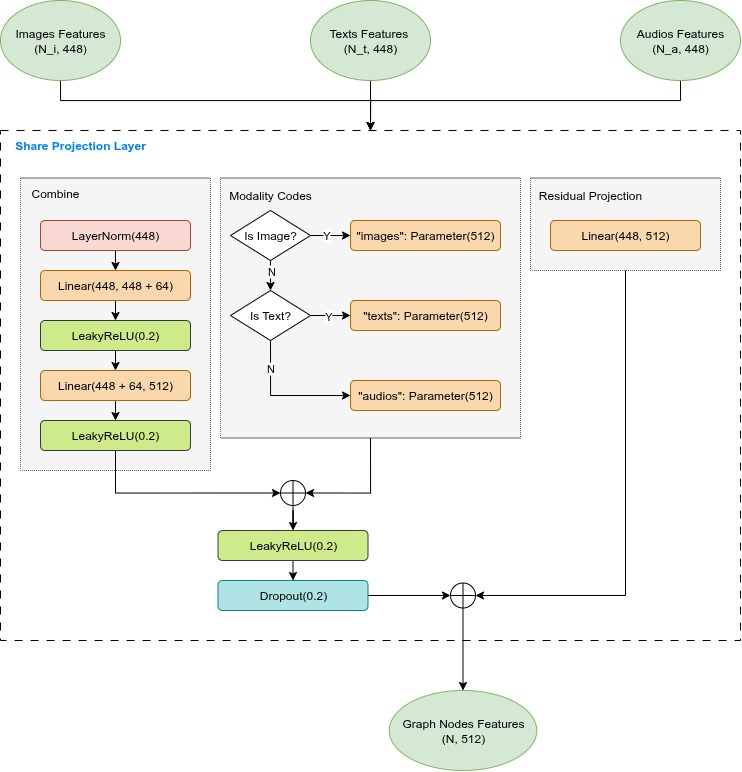
\includegraphics[width=0.8\linewidth]{images/part-02/chap-02/sec-01/ShareProjectionLayer.jpg}
    \vspace{0.3cm}
    \caption{Kiến trúc của Share Projection Layer}
    \label{fig:KTShareProjectionLayer}
\end{figure}

Để mô hình phân biệt được nguồn gốc của từng vector đặc trưng trong không gian chung, hệ thống sử dụng kỹ thuật \textit{Modality Embeddings} (hay Modality Codes). Mỗi phương thức được gán một vector tham số học được riêng biệt, cộng trực tiếp vào đặc trưng đầu ra nhằm ``đánh dấu'' vị trí của nó trong không gian vector chung. Kỹ thuật này được lấy cảm hứng từ cơ chế \textit{Token Type Embeddings} trong mô hình BERT, giúp mô hình nhận biết ngữ cảnh phương thức \cite{devlin2019bertpretrainingdeepbidirectional}. Đồng thời, cơ chế Residual Connection tiếp tục được áp dụng tại đây nhằm duy trì luồng thông tin xuyên suốt, tránh sự mất mát dữ liệu do các phép biến đổi không gian.
%===================================================================
\paragraph{1.2.3. Tầng học trọng số cạnh}
\indent\indent Tầng này đóng vai trò khởi tạo cấu trúc đồ thị bằng cách xác định độ mạnh yếu của các liên kết giữa các đỉnh, như minh họa tại \textbf{Hình \ref{fig:KTEdgeWeightsLayer}}.

\begin{figure}[H]
    \centering
    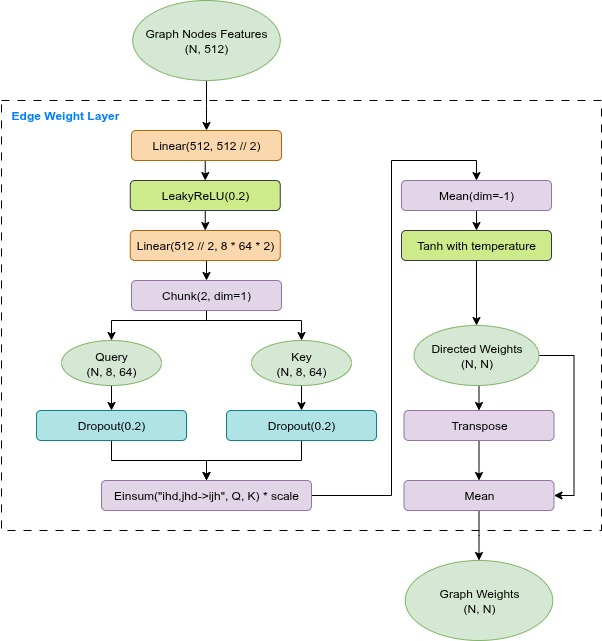
\includegraphics[width=0.8\linewidth]{images/part-02/chap-02/sec-01/EdgeWeightsLayer.jpg}
    \vspace{0.3cm}
    \caption{Kiến trúc của Edge Weights Layer sử dụng cơ chế Attention}
    \label{fig:KTEdgeWeightsLayer}
\end{figure}

Mạng học trọng số được thiết kế dựa trên cơ chế \textit{Self-Attention} với tích vô hướng $Q \cdot K^T$ để nắm bắt tương quan ngữ nghĩa \cite{vaswani2023attentionneed}. Đặc biệt, đầu ra sử dụng hàm kích hoạt \texttt{Tanh} để giới hạn giá trị trong khoảng $[-1, 1]$. Việc cho phép trọng số âm tại bước này đóng vai trò như một cơ chế "lọc mềm" (soft thresholding): các giá trị âm sẽ được quy về 0 bởi hàm \texttt{Clamp(min=0)} ở các tầng tiếp theo, giúp mô hình chủ động học cách ngắt bỏ các kết nối nhiễu hoặc không liên quan thay vì buộc phải duy trì tất cả các cạnh với trọng số dương nhỏ. Bên cạnh đó, để đảm bảo tính vô hướng của đồ thị, tôi thêm vào phép tính trung bình cộng giữa ma trận trọng số với ma trận chuyển vị của chính nó, điều này đảm bảo rằng trọng số kết nối từ đỉnh A đến đỉnh B và ngược lại là như nhau.
%===================================================================
\paragraph{1.2.4. Tầng GAT}
\indent\indent Đây là thành phần cốt lõi thực hiện quá trình truyền tin (Message Passing) để cập nhật đặc trưng đỉnh, với kiến trúc được minh hoạ như \textbf{Hình \ref{fig:KTGATLayers}}.

\begin{figure}[H]
    \centering
    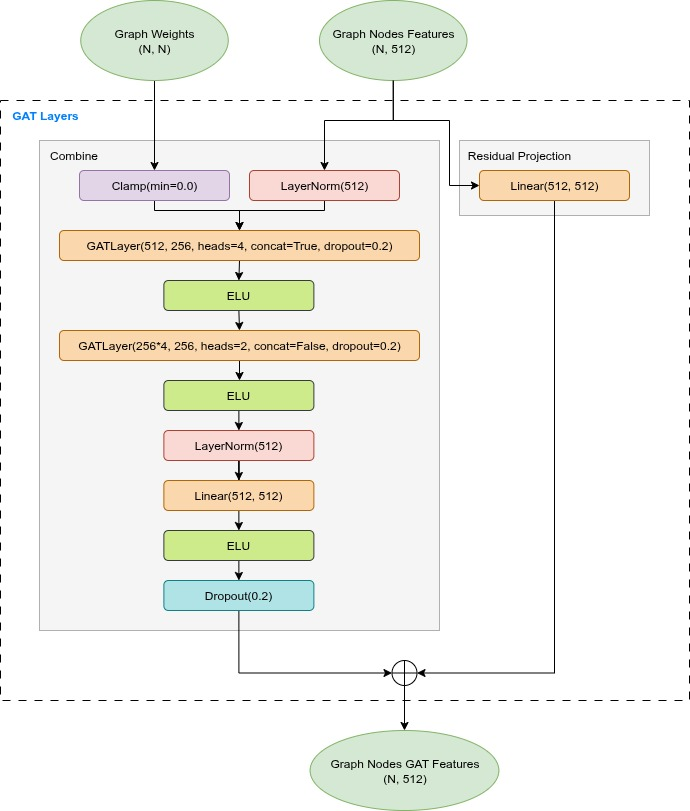
\includegraphics[width=0.8\linewidth]{images/part-02/chap-02/sec-01/GATLayers.jpg}
    \vspace{0.3cm}
    \caption{Kiến trúc của GAT Layers với cơ chế Weighted Message Passing}
    \label{fig:KTGATLayers}
\end{figure}

Hệ thống áp dụng biến thể \textbf{Weighted GAT} kết hợp với \textit{Dynamic Attention}. Khác với GAT truyền thống chỉ dựa vào đặc trưng nút và ma trận kề để tính hệ số attention, thì mô hình của tôi tích hợp trực tiếp trọng số cạnh học được ($GW_{ij}$) vào quá trình tính toán:
\[
    \alpha_{ij} = \text{softmax}(\text{LeakyReLU}(\vec{a}^T [W\vec{h}_i \| W\vec{h}_j]) \cdot {GW}_{ij})
\]
\indent Trong đó $GW_{ij}$ là ma trận trọng số cạnh của đồ thị từ tầng trước đã qua hàm \texttt{Clamp(min=0.0)} để loại bỏ giá trị âm. Cơ chế này giúp khắc phục hạn chế "Static Attention", cho phép mô hình kiểm soát dòng chảy thông tin linh hoạt hơn: các cạnh có trọng số lớn sẽ khuếch đại tín hiệu, ngược lại các cạnh yếu sẽ bị chặn lại. Hàm kích hoạt phi tuyến ELU (Exponential Linear Unit) được sử dụng sau mỗi lớp GAT nhằm hỗ trợ việc học các biểu diễn mạnh mẽ hơn và tăng tốc độ hội tụ so với ReLU tiêu chuẩn \cite{clevert2016fastaccuratedeepnetwork}.\vspace{0.3cm}

Ngoài ra, tại tầng này tôi sử dụng thêm kỹ thuật \textit{Pre-LayerNorm} (chuẩn hóa trước khi đưa vào layer) để ổn định gradient khi huấn luyện mô hình sâu, tránh hiện tượng bùng nổ hoặc triệt tiêu gradient thường gặp trong các mạng GNN nhiều lớp \cite{xiong2020layernormalizationtransformerarchitecture}. Tương tự các tầng trước, cơ chế Residual Connection vẫn được duy trì để bảo toàn thông tin gốc qua các phép biến đổi phức tạp.
%===================================================================
\paragraph{1.2.5. Bộ phân lớp}
\indent\indent Tầng cuối cùng thực hiện ánh xạ từ không gian đặc trưng đồ thị sang không gian nhãn xác suất, sử dụng tùy chọn FastKAN hoặc MLP như minh họa tại \textbf{Hình \ref{fig:KTClassifier}}.

\begin{figure}[H]
    \centering
    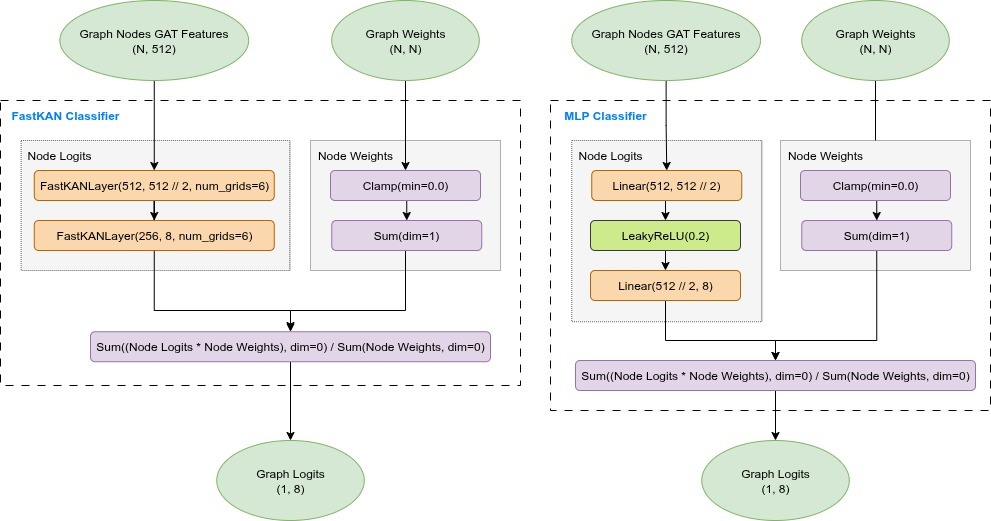
\includegraphics[width=\linewidth]{images/part-02/chap-02/sec-01/Classifier.jpg}
    \vspace{0.3cm}
    \caption{Kiến trúc bộ phân lớp bằng FastKAN và MLP}
    \label{fig:KTClassifier}
\end{figure}

Thay vì sử dụng kỹ thuật \textit{Global Mean Pooling} thông thường (coi vai trò các đỉnh là như nhau), tôi áp dụng cơ chế \textit{Weighted Voting (Bầu chọn có trọng số)}. Kết quả dự đoán cuối cùng là trung bình có trọng số của các dự đoán từ từng đỉnh ($logits_i$), dựa trên tổng trọng số kết nối dương ($d_i = \sum_j w_{ij}$) của đỉnh đó:
\[
    y_{pred} = \frac{\sum_i (logits_i \cdot d_i)}{\sum_i d_i + \epsilon}
\]
\indent Trong đó $\epsilon$ là hằng số nhỏ để tránh lỗi chia cho 0. Cơ chế này phù hợp với lý thuyết về \textit{Graph Readout Operations}, khẳng định rằng việc tổng hợp thông tin dựa trên cấu trúc giúp mô hình ưu tiên các đỉnh trung tâm giàu thông tin và giảm thiểu tác động của các đỉnh nhiễu ngoại lai \cite{xu2019powerfulgraphneuralnetworks}.